\section{Experimental Results}
\label{Experimental Results}

We used the simulator to examine the results of the game between teh adversary and the utility described in Section \ref{Game}.  We examined the effectiveness of our four propowed adverserial strategies and our suggested defense techniques under two different scenarios.  In the first, there are an equal number of each class of customer.  In the second, 40\% are Bakeries, 40\% are Batteries, and the remaining 20\% are Buckets.  In both scenarios we assume that the attacker and the utility have the same budget, ie they can attack / defend the same number of customers.  All of our results are over 15,000 total customers in order to make our distribution assumptions accurate.  Further the results presented here are averaged over 10 different random number seeds in order to eliminate any bias in a given sample from the distributions.  The results are presented relative to the mismatch achieved by the scheduling algorithm without an adversary.    

\begin{figure*}[htp]
    \centering
    \subfigure[Scenario 1]{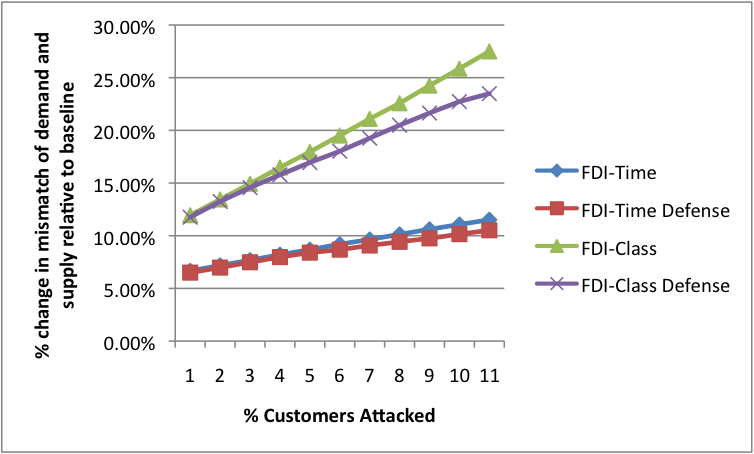
\includegraphics[width=.5\textwidth]{naieve-equal-attacks.png}}\hfill
    \subfigure[Scenario 2]{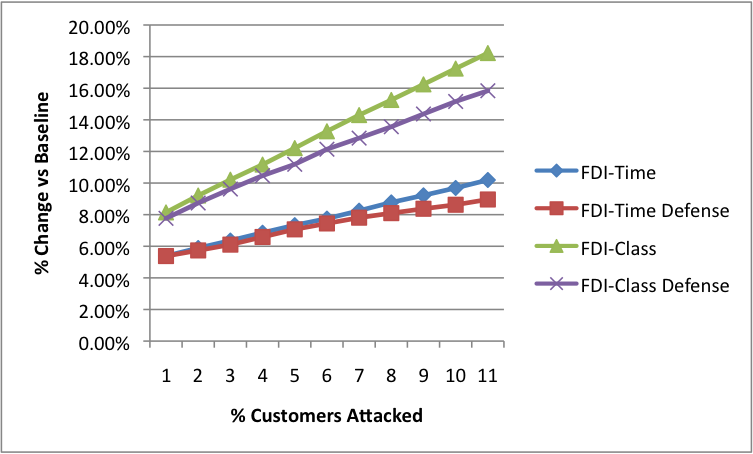
\includegraphics[width=.5\textwidth]{naieve-unequal-attacks.png}}  
    \caption{Results for Naieve Attacker}
    \label{naieve}  
\end{figure*}

We first considered a naieve attacker who targets all customers independently.  In this case neither the Jamming nor the FDI-Load attack had any significant effect, and so are ommitted from Figure \ref{naieve}.  Our defense is relatively ineffective against the naieve attacker, because it is hard to defend against randomness.  However, the attack itself is also far less effective: only increasing the mismatch by 28\% in the worst case versus 52\% for the strategic adversary.

Given this naieve baseline, we examined how much more effective a \emph{strategic} adversary is.  In particular, the adversary targets bakeries for all attacks other than the FDI-Class where it targets buckets.  These are the types of customers where the attack is most potent, as our results in Figure \ref{strategic} show.

\begin{figure*}[htp]
    \centering
    \subfigure[Scenario 1]{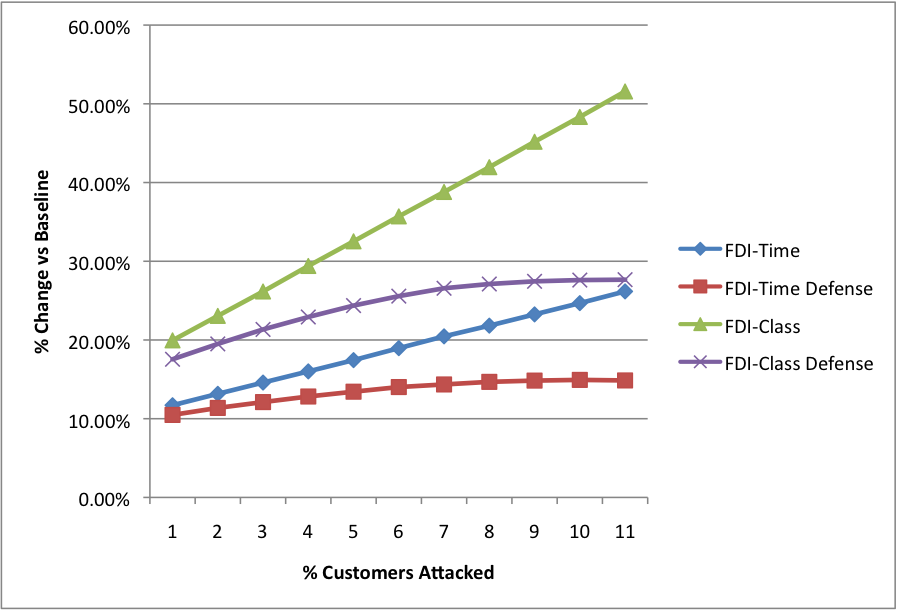
\includegraphics[width=.5\textwidth]{equal-attacks.png}}\hfill
    \subfigure[Scenario 2]{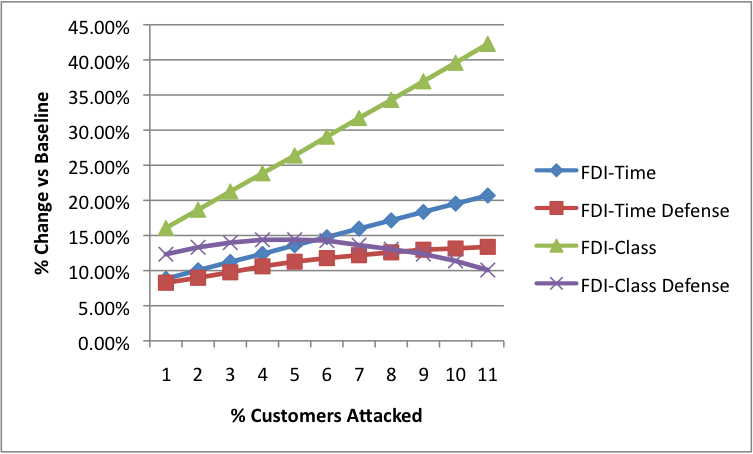
\includegraphics[width=.5\textwidth]{unequal-attacks.png}}  
    \caption{Results for Naieve Attacker}
    \label{naieve}  
\end{figure*}

Again, the FDI-Load and Jam attacks are too constrained to be effective, and are ommitted from our results.  However, the strategic attack has a significant impact, increasing mismatch by 52\% in the worst case.  However, our defense was able to blunt the strategic adversary back down to the efficacy of the naive, random adversary.  This is a significant decrease: dropping the additional attacker induced mismatch from 52\% of baseline to 28\% of baseline. 

The other notable result is that the efficacy of our defense against the FDI-Class attack \emph{increases} as more customers are attacked.  This attack targets Buckets, the most flexible type of customer, and turns them into Bakeries, the least.  The efficacy of our defense, which preserves Buckets, underscores the critical nature of the flexibility they provide ot the utility.  

